\chapter{Design}

To recap, this project used a hybrid approach of a plan-driven methodology followed by an agile implementation. The design stage is where the first methodology began to merge into the other.

A lot of time was invested in clarifying requirements so that the common classes and methods could be established and fed into parts of the initial design. As a result, certain aspects of the design could be designed up front as they were unlikely to change unless there was a change in requirements. Other aspects such as class diagrams would not be suitable for up front design, since the code would be refactored throughout the process and would ultimately fall out of line with the documentation.

\section{Development choices}

\subsection{Programming language}

As a web-based solution, the options were somewhat constrained to server-side languages. PHP, Node and Ruby on Rails all came to mind. It was decided that PHP would be the most appropriate choice.

PHP is currently the most popular server-side programming language worldwide, and, perhaps more importantly, it's the server-side language I had by far the most experience using.~\cite{phpPopular} My thought process was this: though I could have spent a few weeks learning the intricacies of ASP.NET to deliver my project, it would have been an unwise use of my time given that there was so much to build. I didn't want to find myself desperately trying to debug an obscure error in an unfamiliar language a week before the deadline.

Development experience aside, PHP being the most popular server-side language means that there is extensive support and documentation online: any problems faced during development have likely already been solved through other peoples' experiences. Moreover, if the project were to go open-source, it would be more likely to acquire a sizeable and active developer community than a lesser-known language. Finally, server-support for PHP is very common: by opting for PHP as the language of choice, SmartResolution is more likely to be able to be installed and used by more people.

\subsection{BDD Framework}

There are many options for parsing feature files. Cucumber was originally built for Ruby, but now there are other variants such as CucumberJS (for JavaScript) and Lettuce (for Python). The de facto standard BDD implementation for PHP is Behat.

Personally, I dislike Behat because of its syntax. It requires that you define your step definition as a concatenated function name and write metadata above the function definition:

\begin{minipage}{\textwidth}
\begin{lstlisting}[language=php]
/**
* @Given /^I am in a directory "([^"]*)"$/
*/
public function iAmInADirectory($argument1)
{
throw new PendingException();
}
\end{lstlisting}
\end{minipage}

This just isn't as \emph{clean} as Cucumber and Ruby:

\begin{minipage}{\textwidth}
\begin{lstlisting}[language=ruby]
Given(/^I am in a directory (.+)$/) do |argument|
# pending
end
\end{lstlisting}
\end{minipage}

Syntactical disagreements aside, Matthew Daly's blog post about testing PHP web applications with Cucumber discusses the benefits of Ruby and Cucumber compared with Behat. He opts for the former because RubyGems makes it easy to install Cucumber's dependencies and the Cucumber community appears to be very active.~\cite{matthewDaly}

Finally, by choosing a BDD framework whose language is different to that of my project, I'd be forcing decoupling between my application and its regression tests, making it impossible to make certain inappropriate testing choices such as directly including application PHP classes inside the step definitions. For all of the reasons outlined above, I decided to opt for Ruby and Cucumber as my BDD framework.

\subsection{Reusing open-source software}

It was hoped that there would be an existing open-source ODR platform upon which to base the project. One would have been able to make the necessary modifications to support the maritime collision module without having to build the entire platform from scratch, thus allowing more time to be spent on the maritime collision module.

Unfortunately, after fairly extensive research, I was unable to find an existing ODR platform that was not proprietary. Most ODR providers, be they service or platform providers, charge a subscription or one-off fee and would be at a commercial disadvantage if they were to go open-source. Without an existing ODR platform to base the project upon, there was no option but to develop the core platform from scratch.

\subsection{Project Framework}\label{subsection:framework}

It makes sense to minimise development effort through the use of a framework, letting the combined efforts of hundreds of contributing developers do the heavy lifting so that we are free to implement the application-specific code. Dozens of PHP frameworks exist, so deciding on one can be difficult.

Large frameworks such as Zend and Symphony are quite constraining, requiring you to stick to their idea of what is the best development approach or else perform some very heavy, non-standard configuration to make it suit your project. Either of these heavyweight frameworks could be perfectly well suited to ODR, but generally speaking I try to stay away from non-transferable frameworks. I like to understand exactly how my application works, rather than delegate that understanding to a third-party library. It is also advantageous to be able to change frameworks painlessly at a later date - something which is not suited to heavyweight frameworks.

Lighter options exist, including Huge, Laravel and Fat-Free Framework. Huge looked promising to begin with but then appeared to be more of a middleweight framework, strongly encouraging certain directory structures. It would be a base that the ODR software would have to build upon, rather than a library that could be plugged into the system, only called as and when needed.

Laravel was the next one considered and looked a little like PHP's answer to Rails, as it generates an entire application structure through a single command. Again, this framework comes with a set of defaults which may not necessarily be suited to your project, locking you into a pre-conceived idea of how an application should be structured.

It would be impossible to thoroughly evaluate every framework to make a truly considered decision, and I'm sure that any one of the above frameworks would have been a perfectly suitable starting point. However, the most promising-looking framework for an agile project was Fat-Free Framework, or F3 as it is commonly known. It had a low learning curve and an unconstraining nature, and its modular build meant that I could cherrypick the elements of functionality needed for the project, rather than go for an all-or-nothing installation. F3 is fundamentally different to its competitors because I could slot F3 into my code, rather than slotting my code into F3. For these reasons, I chose F3 as SmartResolution's framework.

In a recent interview I presented this argument to Gavin Love, Chief Technology Officer at MyBuilder.com, who agreed that modularity seems to be the way that PHP frameworks are heading. This suggests that delegating units of functionality to a lightweight framework might be a future-proof decision. Developing software on a heavyweight framework which subsequently loses support can be very difficult to refactor, as Gavin says he found when upgrading MyBuilder.com from Symphony 2 to Symphony 3.

\section{Overall architecture}

The project can be broken down into three main components.

\subsection{Core platform}

SmartResolution is the ODR platform offering the core online dispute resolution requirements, such as organisation and user registration, dispute creation, messaging, file uploads, and so on. It offers the minimum facilities necessary to successfully negotiate a dispute online.

As this was the basis of all the other components, it was also the most thoroughly engineered, backed up with integration and unit tests, continuous integration, automated code quality checks and dependency status checks.

\subsection{Maritime collision module}

This module is separate from the core platform and lives in its own repository. It can be manually installed to any SmartResolution installation simply by being copied to the \lstinline{modules} directory, or automatically installed through the SmartResolution Marketplace facility.

As discussed in the background and initial requirements, it was intended for this to be a feature-rich module that could find similar historic cases, cross-check agents' answers with maritime law, and approximate the likelihood of an agent's success in court.

\subsection{SmartResolution Marketplace}

smartresolution.org is the vendor site for SmartResolution, explaining what SmartResolution is and offering a download link to a production-ready version. Its subdomain, demo.smartresolution.org, has a live demo of the SmartResolution software installed so that users can try out the software before they download. However, one of the main reasons for developing the website was the creation of the `marketplace' facility, discussed later in this chapter.

\section{WordPress: a comparison}

The commercial viability of the software (analysed in appendix~\ref{appendix:commercialViability}) drew some parallels with the blogging software WordPress. WordPress can be said to have a three-tier system:

\begin{enumerate}
    \item \textbf{WordPress platform}: blogging software that can be downloaded, installed and hosted on a LAMP server.

    \item \textbf{WordPress plugin}: a self-contained package that can be installed to a WordPress installation and which augments the core installation with additional functionality.

    \item \textbf{Plugin Directory}: a searchable area of the WordPress.org website which links to thousands of available plugins. This facility is tightly coupled to the administrative functions in the core software, as administrators are able to browse, download and install plugins from wordpress.org, within the WordPress installation itself.
\end{enumerate}

These three tiers map to the SmartResolution core platform, the maritime collision module and the SmartResolution Marketplace respectively.

Some developers can be quite narrow-minded about WordPress, but it is a platform that powers 23\% of the internet.~\cite{wordpressPopular} The reasons for this are that it is open-source, highly customisable, and the developer documentation is very good. The brand is reliable: people trust it. I will try to emulate all of this as much as possible in the development of SmartResolution.

\section{Choice of Licenses}

The design section may seem an incongruous place to discuss the issue of licensing, but licensing can be thought of as a high-level form of design. Linus Torvalds, chief architect of the Linux kernel, once said he considered his choice of the GPL license for the Linux kernel ``one of the very best design decisions" he made, since it is designed to protect the author's legal and moral rights to their code.~\cite{linusLinux}

I opted for the GPLv3 license for the core SmartResolution software. This is almost identical to WordPress' choice of a GPLv2 license, which is presumably still at version 2 for legacy or backwards-compatibility reasons.

The benefits of a restrictive license is that nobody has the ability to download, modify and then sell the software without making the source available to all. Multinational corporations who can afford to compensate developers for their time are not able to use SmartResolution as a basis for closed-source software\footnote{This only applies if the company is \emph{distributing} the software. In-house software can remain closed-source.}. Any improvements they make to the software must be kept open-source, as it is a derivative work.

On the other hand, the GPL allows for legitimate use-cases for SmartResolution. For instance, anyone can download the software, install it on their own server and start providing ODR services. They can even charge a subscription fee, and would owe nothing to the SmartResolution developers. The choice of GPLv3 for SmartResolution protects me from other people making money selling \emph{software} derived from this project. It doesn't stop people making money providing ODR as a service, and it won't infect their website ``like a cancer", to quote Steve Ballmer, ex-CEO of Microsoft.~\cite{linuxCancer}

Though I originally hoped to release the maritime collision module under the MIT license, WordPress and Drupal believe strongly that any plugins or themes for their CMS are classed as derivative works, stating: ``The GPL on code applies [also] to code that interacts with that code".~\cite{wordpress:gpl} Thus, like the parent software, these derivatives should be bound to a GPL-compliant license. Any modules which call PHP functions defined by the core SmartResolution software must therefore also be bound to the GPL license, so I have released the module under the GPLv3 license.

The fact that all distibuted modules are bound to the terms of the GPL shook my confidence in the commercial viability of creating proprietary modules for the system. I found it difficult to understand how WordPress' premium plugins were able to be sold at all, as one of the four freedoms enabled by the GPL is ``the freedom to redistribute copies", meaning anybody who purchases a premium WordPress plugin is able to redistribute the plugin for free.~\cite{fourFreedoms} Chris Lema suggested a number of explanations for the success of premium plugins in his blog post, mainly alluding to the fact that only plugins which are bought legitimately get the latest updates, bug fixes and support for a specific period of time.~\cite{chrisLema} The fact that so many plugins and themes \emph{are} able to be sold through WordPress indicates that the same business strategy could be applied to SmartResolution modules.

I saw no advantage in making the SmartResolution website itself open-source, since I'm not encouraging anybody to download and re-use the website itself. I have kept the source-code for smartresolution.org private and all of its contents are under my copyright.

\section{Design: SmartResolution}

\subsection{Choice of Database Management System}

Before going down the route of designing a database schema, a decision had to be made as to whether to go for a relational database management system (RDBMS) or an object-oriented database management system (OODBMS). The former is the traditional means of application persistence, whereas the latter is still fairly new and is intended to allow developers to think purely in terms of object-orientation.

RDBMSs have more widespread support than OODBMSs, and I wanted SmartResolution to be as accessible as possible for those wanting to provide their own ODR services. In addition, my choice of PHP framework has built-in database support and is geared towards relational databases.

OODBMSs gives an advantage to those companies that are geared towards multimedia presentation or organizations that utilize computer-aided design.~\cite{oodbms} In contrast, SmartResolution is quite text-heavy and is perfectly well suited to a RDBMS implementation.

My next decision was which RDBMS to go for. The market leader is MySQL, but many alternatives exist, such as PostgreSQL, MSSQL, Oracle and SQLite. F3 supports all of these and more.~\cite{f3:sqlConstructor} The quickest database to get started with was SQLite, as it meant that I could develop locally without having to worry about creating the database administrator accounts required by other RDBMSs, such as MySQL. SQLite databases exist simply as a file on the system, whose contents can be viewed and edited through a program such as DB Browser for SQLite. The fact that SQLite databases exist as files on the system makes having multiple databases trivial, so my system can easily switch between test and production databases depending on the context in which the application is accessed. For these reasons, I selected SQLite as the RDBMS of choice for the project.

It is important to note that this can be swapped out for another RDBMS relatively easily, since all database interactions in SmartResolution go through one \lstinline{Database} class. This class calls F3's \lstinline{SQL} class, and as discussed above, F3 has implementations for all of the main RDBMSs. Indeed, if I had a SmartResolution installation in a production environment which was being used by thousands of people, I would consider changing to a RDBMS such as MySQL. Even the SQLite developers suggest that SQLite is best suited as a stand-in for an enterprise RDBMS: ``SQLite is often used as a surrogate for an enterprise RDBMS for demonstration purposes or for testing".~\cite{sqliteFeatures}

\subsection{Database schema}

\begin{figure}[h!]
  \centering
    \ifimages
    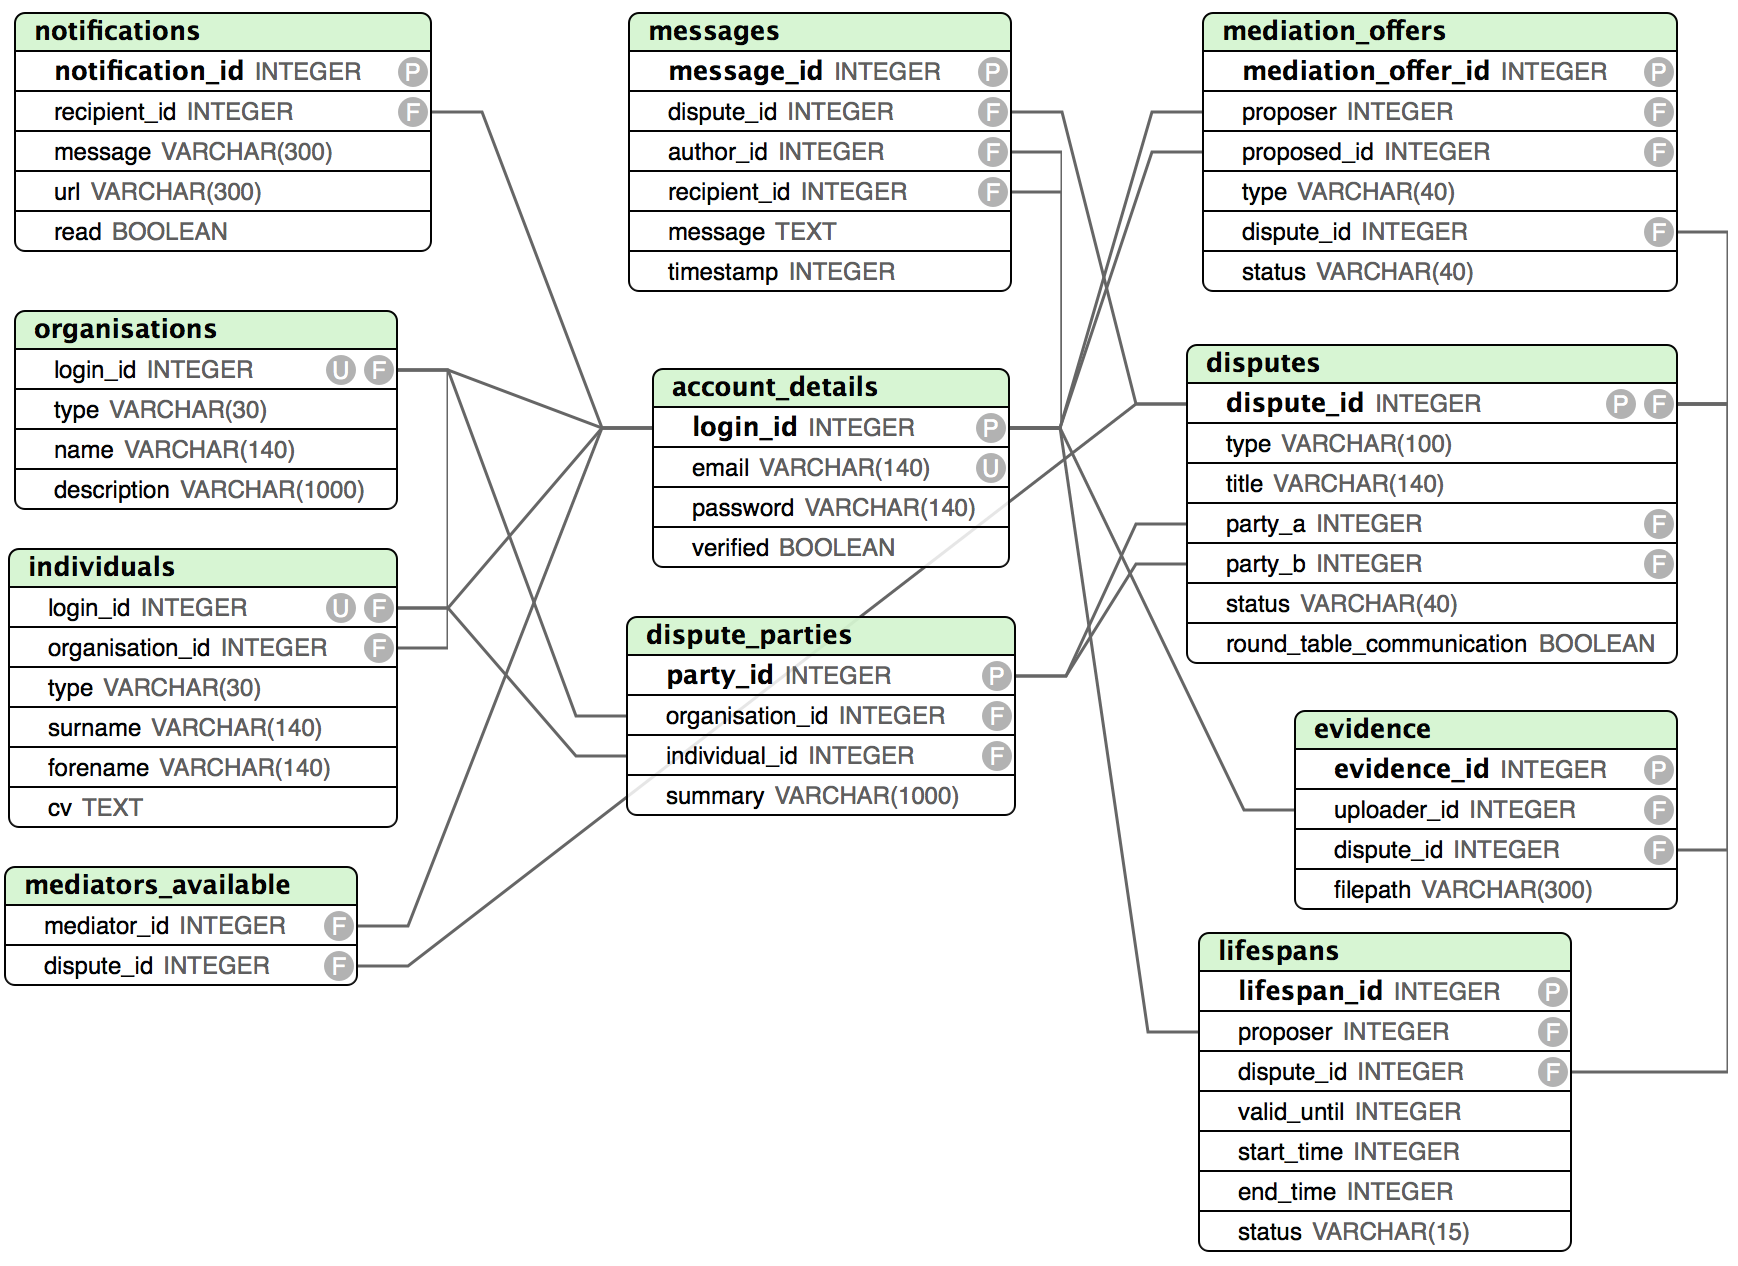
\includegraphics[width=\textwidth]{database}
    \fi
  \caption{Database schema for the SmartResolution core platform}
  \label{uml:databaseSchema}
\end{figure}

Figure~\ref{uml:databaseSchema} shows the database schema for the SmartResolution core platform, where \lstinline{P} symbols refer to primary keys, \lstinline{F} symbols refer to foreign keys, and \lstinline{U} symbols refer to unique integrity constraints. Lines generally denote foreign key relationships. Other integrity constraints exist, such as `organisations.type' only being one of ``law\_firm" or ``mediation\_centre". These have been omitted from the diagram.

For a full explanation and justification of the database design, please refer to appendix~\ref{appendix:database}.

\subsection{Module support}\label{subsection:moduleSupport}

This section of work is separate from the maritime collision module work, and is concerned with how the core platform should support modules at an abstract level. There should be no maritime-collision-specific code in the core SmartResolution platform, but the platform must support all functionality required by the module.

Taking inspiration from WordPress' Plugin API, the project uses the concept of `hooks' in a publish-subscribe design pattern. WordPress fires events at various points throughout the normal running of a WordPress installation; these events can be subscribed to and a custom function executed to achieve some arbitrary purpose.

For example, below is WordPress' \lstinline{add_filter} function:

\begin{lstlisting}[language=php]
add_filter('img_caption_shortcode', 'my_filter', 10);
\end{lstlisting}

The first argument is the event to listen for, the second argument is the custom function to execute, and the third argument is an integer denoting the priority of our subscription. Subscriptions with a higher priority are executed before those of a lower-priority. SmartResolution fires hooks which can be subscribed to in the same way as the WordPress function above.

F3's routing API can extend this route-handling concept further:

\begin{lstlisting}[language=php]
$f3->route('GET /some-route' => 'MyClass->handler');
\end{lstlisting}

F3's routing allows the developer to assign handling to a public method of a class, rather than a global function, keeping the codebase namespaced and tidy. This is something I've carried over to SmartResolution's parsing of the function name.

These principles formed the basis for the design of the module support:

\begin{lstlisting}[language=php]
on('event', 'function_to_call', 'priority');
\end{lstlisting}

`event' is the name of the event to subscribe to, `function\_to\_call' is the name of the function to call (and can be a global function, a named class function or an anonymous function), and `priority' represents the priority with which the function should be called. The priority can be an integer or a string such as `high', `medium' or `low'.

\subsection{Exposing other methods}

One needs to be able to manipulate the rendered output of SmartResolution, e.g. when adding a menu item to the dashboard of a dispute.

This \emph{could} be accomplished by interacting directly with the core platform, as in the example below.

\begin{lstlisting}[language=php]
global $dashboardActions;
$item =  array(
    'title' => 'Some Action',
    'image' => get_module_url() . '/images/icon.png',
    'href'  => get_dispute_url() . '/custom-route'
);
array_unshift($dashboardActions, $item);
\end{lstlisting}

This example encourages tight coupling between the module and the underlying platform, locking the core platform into a particular design and risking breaking backwards compatibility should SmartResolution be refactored in the future. If the \lstinline{$dashboardActions} global variable was removed from the core platform, or the dashboard actions represented with something other than an array, it would break any existing modules relying on that specific implementation.

Again, WordPress provided inspiration for the design. WordPress exposes a number of global functions, e.g. \lstinline{get_the_id}, which gets the ID of the current post. In this style, SmartResolution exposes a number of global functions. One could now manipulate the rendering of the dashboard like this:

\begin{lstlisting}[language=php]
dashboard_add_item(array(
    'title' => 'Some Action',
    'image' => get_module_url() . '/images/icon.png',
    'href'  => get_dispute_url() . '/custom-route'
));
\end{lstlisting}

Not only does this decouple the module/SmartResolution interaction, but this is much cleaner and easier from the module developer's perspective. It is important that there should be as few barriers as possible when it comes to module development, if developers are to get excited about SmartResolution.

\subsection{Module persistence}

Persistence was the most difficult area to tackle, as interacting with the database introduces persistent changes which could be harmful if the developer is not careful. On the one hand, the system has to trust developers. Regardless of the database access methods explicitly exposed by the underlying system, there's nothing stopping developers from accessing the global \lstinline{Database} class used by the core platform, especially since SmartResolution is open-source and the developer can easily find out what system-level classes are available. At an even lower level, there's nothing stopping a developer from running PHP's \lstinline{shell_exec} function and executing any command they wish.

The system should trust developers, but it should not trust developers to write perfect code. Though most developers would use an SQL-execution ability only for querying the database for a legitimate reason, they may expose a vulnerability if not thoroughly tested. For example, if they're writing a search engine module which takes a user input, and if they do not sanitise the query, then they're letting the \emph{end user} run arbitrary SQL.

With security in mind, it was decided that the global function definitions should be expanded to define functions supporting specific SQL interactions, e.g. creating tables, selecting rows, updating records, and so on. Early on it was tempting to allow table schema updates on the fly, creating columns as and when they were needed, but this felt dangerous and was tricky to implement. I settled on an up front table design solution by way of a \lstinline{declare_table} function:

\begin{lstlisting}[language=php]
declare_table('my_table', array(
    'a_text_field' => 'TEXT NOT NULL',
    'an_int_field' => 'INTEGER DEFAULT 0',
    'initiated'    => 'BOOLEAN'
));
\end{lstlisting}

The newly created table can then be inserted into and queried using specific, named functions. This does somewhat restrict what the developer can do - for example, there is no method for doing SQL table joins - but more often than not, the developer can still achieve what they need to achieve using pure application code.

In the above example, \lstinline{my_table} is not the name of the created table. Instead, it is namespaced as \lstinline{module__[module_name]__my_table}. The module developer doesn't need to know this, and can continue to refer to \lstinline{my_table} in all of their queries as if that is the name of the table. This means we have the advantage of namespacing our tables (preventing naming conflicts where different modules use common table names) but without the technical overhead of having to rememember to prefix table names with that namespace.

Most modules will require some sort of persistence layer to be useful, but developers are not necessarily locked into this database setup. They could use PHP's \lstinline{file_put_contents} to save to a file, perhaps in conjunction with \lstinline{json_encode} to save a PHP array as a JSON file. They could even use PHP's \lstinline{shell_exec} command to create a new SQLite database in their module's directory, giving them complete freedom and the responsibility it comes with. The database functions offered by SmartResolution cut out some of the complexity of doing persistence from scratch, but are by no means the only way of storing data persistently.

\section{Design: Maritime collision module}

This module was developed in tandem with the module support in the core platform. As such, it uses most of the events and hooks exposed by the platform.

As discussed in the requirements section, the basis for the business logic in this module would be the \emph{Convention for the Unification of Certain Rules of Law with respect to Collisions between Vessels}. Everything that is required to apply the Convention can be gathered from a few simple questions, visualised in the flowchart in figure~\ref{uml:maritimeLogic}.

\begin{figure}[h!]
  \centering
    \ifimages
    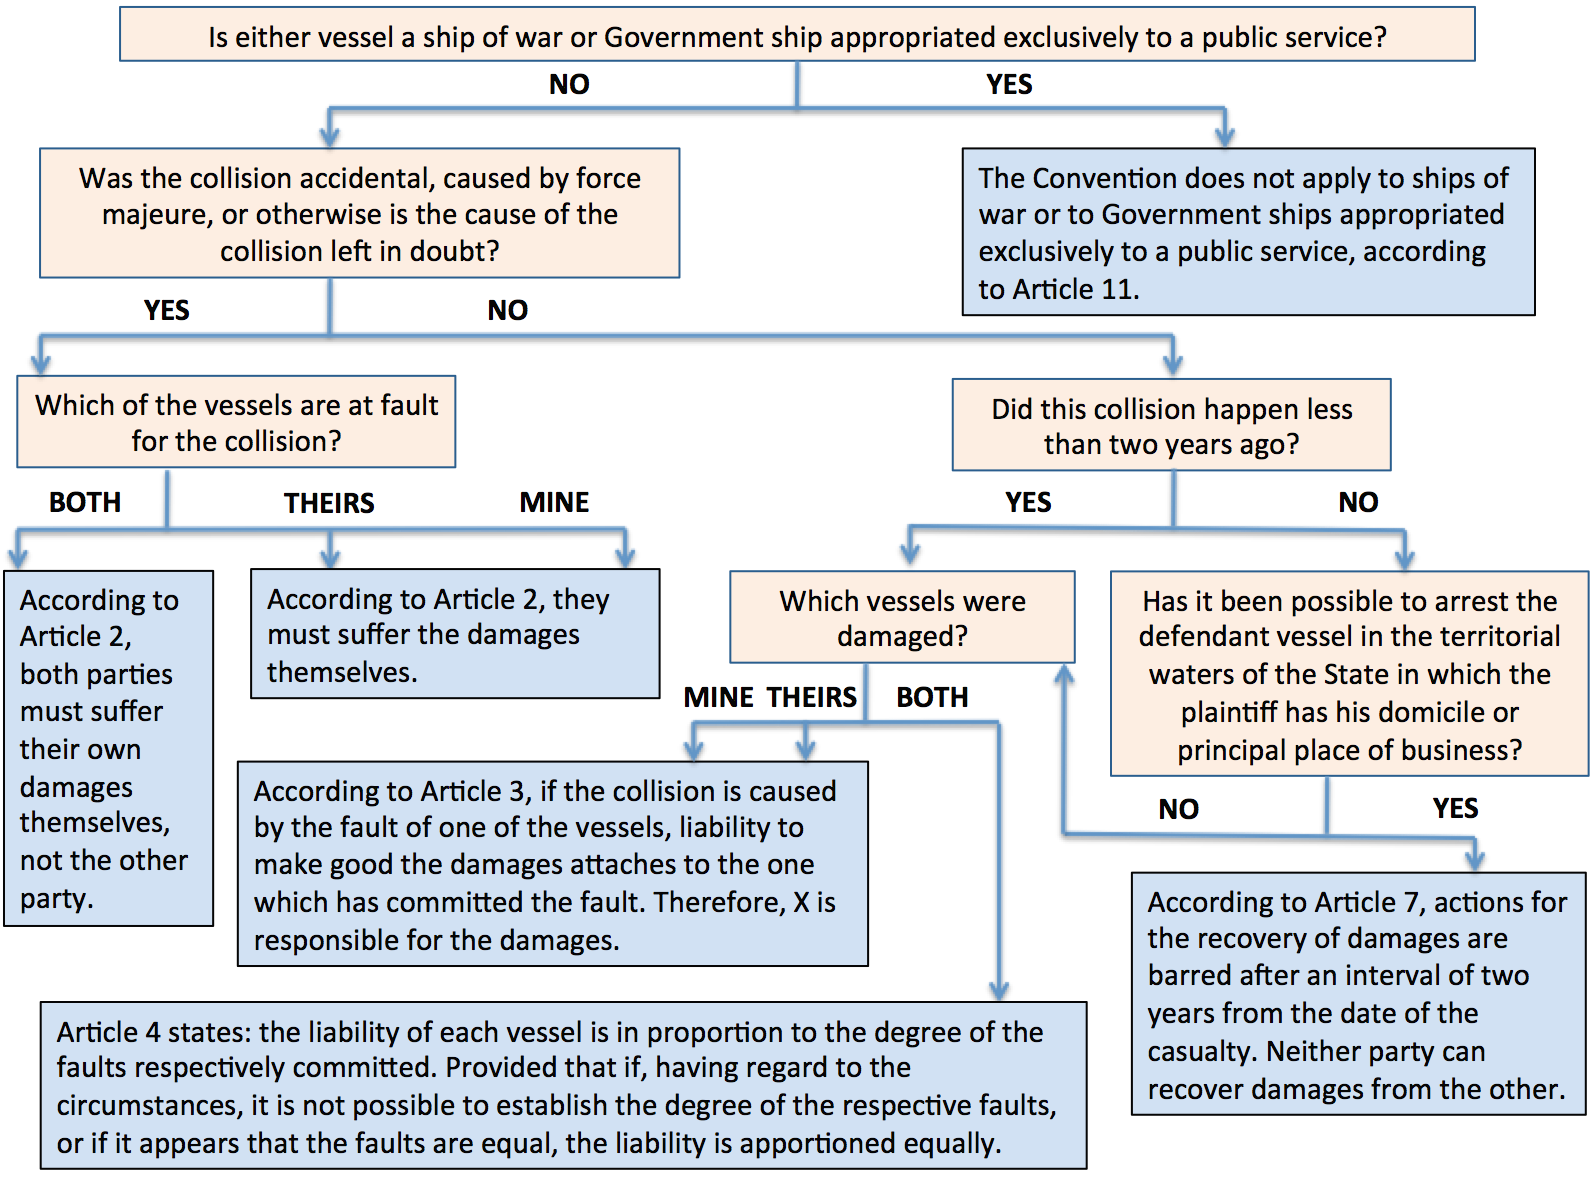
\includegraphics[width=\textwidth]{maritime_collision_logic}
    \fi
  \caption{Logic for Maritime Law results}
  \label{uml:maritimeLogic}
\end{figure}

Some of the business logic is encapsulated in the JSON representing the questions. For example, some questions should only be displayed if certain prerequisites are satisfied. The questions are represented in the following format:

\begin{minipage}{\textwidth}
\begin{lstlisting}
    {
        "prerequisites": [
            {
                "question_id":     "article_11",
                "required_answer": "no"
            }
        ],
        "id":   "article_1",
        "text": "Which vessels were damaged?",
        "type": "select",
        "options": [
            {
                "text" : "The vessel of my client",
                "value": "mine"
            },
            {
                "text" : "The vessel of the other party",
                "value": "other"
            },
            {
                "text" : "Both vessels",
                "value": "both"
            }
        ]
    }
\end{lstlisting}
\end{minipage}

In the above example, the question whose id is \lstinline{article_1} (corresponding to Article 1 of the Convention) is only displayed if the agent answers the question whose id is \lstinline{article_11} with the answer ``no".

When the agents have answered all of the relevant questions, the following happens:

\begin{itemize}
    \item The answers are compared to make sure they tally. If one agent says both vessels were damaged and the other agent says only their vessel was damaged, the answers do not correspond and a conclusion cannot be reached. The module cannot be expected to cope with conflicting information. The module would inform the agents of this.
    \item Provided both answers correlate, the module's \lstinline{ResultsCalculator} class makes a call to the \lstinline{deduceSummary} method, which contains the hard-coded maritime law logic. A resolution is then presented to the agents.
\end{itemize}

Due to the lack of time, the resulting module is a little simplistic. The resolution suggested by the module is deduced through a simple series of if/else statements and probably doesn't tell lawyers anything about maritime law that they don't already know.

However, over-examination of the maritime collision module would be missing the point, which is that the core platform supports any arbitrary module. Modules can be as big and complex as time allows. To go back to the WordPress analogy, on one end of the scale there are many single-file plugins that satisfy a lone developer's personal itch. On the other end, there are enterprise-level plugins that have taken months to engineer and which extend the WordPress platform to be a feature-rich online shop or forum. Given more time, the maritime collision module could be much more heavyweight than it is, encompassing many more aspects of maritime law.

\section{Design: SmartResolution Marketplace}

Early versions of SmartResolution used a PHP array to describe which modules were installed and whether or not they were active. A more user-friendly solution was the creation of an admin dashboard: the ability to sign into an administrator account on your SmartResolution installation, view the installed modules, and activate/deactivate them through a user interface. Following on from this is the ability to view a list of modules, pulled in from smartresolution.org, and download and install them directly through SmartResolution, like WordPress does with plugins.

To accomplish this, there is a JSON feed of featured modules on smartresolution.org\footnote{The JSON feed is viewable at \url{http://smartresolution.org/marketplace/feed}}. This feed is pulled in and converted to HTML, both directly on the marketplace itself\footnote{The human-friendly marketplace is available at \url{http://smartresolution.org/marketplace}} and the SmartResolution admin marketplace dashboard option, emulating what WordPress does with its plugins.

From the admin dashboard on SmartResolution, the modules JSON feed is converted into a HTML page, and server-side logic detects whether or not the module is already installed. If not, a button is rendered which allows the downloading and installation of the module in one click.

In addition to the `Marketplace' admin option, there is a `Modules' option which lists all of the installed modules and whether or not they are active. From this screen, the admin can activate, deactivate or delete the module from their SmartResolution installation.

The ability to define which modules to display externally on smartresolution.org gives the SmartResolution maintainers the freedom to change the contents of that JSON, and therefore change which modules are presented to administrators of SmartResolution installations, irrespective of the version of SmartResolution they have installed. This presents a commercial opportunity, allowing smartresolution.org to categorise paid-for modules as `featured', as hinted by the ``Coming soon" modules for Divorce and Breach of Contract.

\section{User interface}

Bootstrap was used to set up much of the initial design defaults in the core SmartResolution platform and also provides a basic UI framework for the layout. Bootstrap has a 12-column layout requiring a specific HTML structure and class-naming convention, but it does mean that the theme has some built-in responsiveness by default.

The CSS overrides provide a clean and attractive look, and helper classes such as \lstinline{bg-info} and \lstinline{bg-danger} allowed me to style error messages and other components with minimal effort, meaning I could spend more time on the server-side logic.

\begin{figure}[h!]
  \centering
    \ifimages
    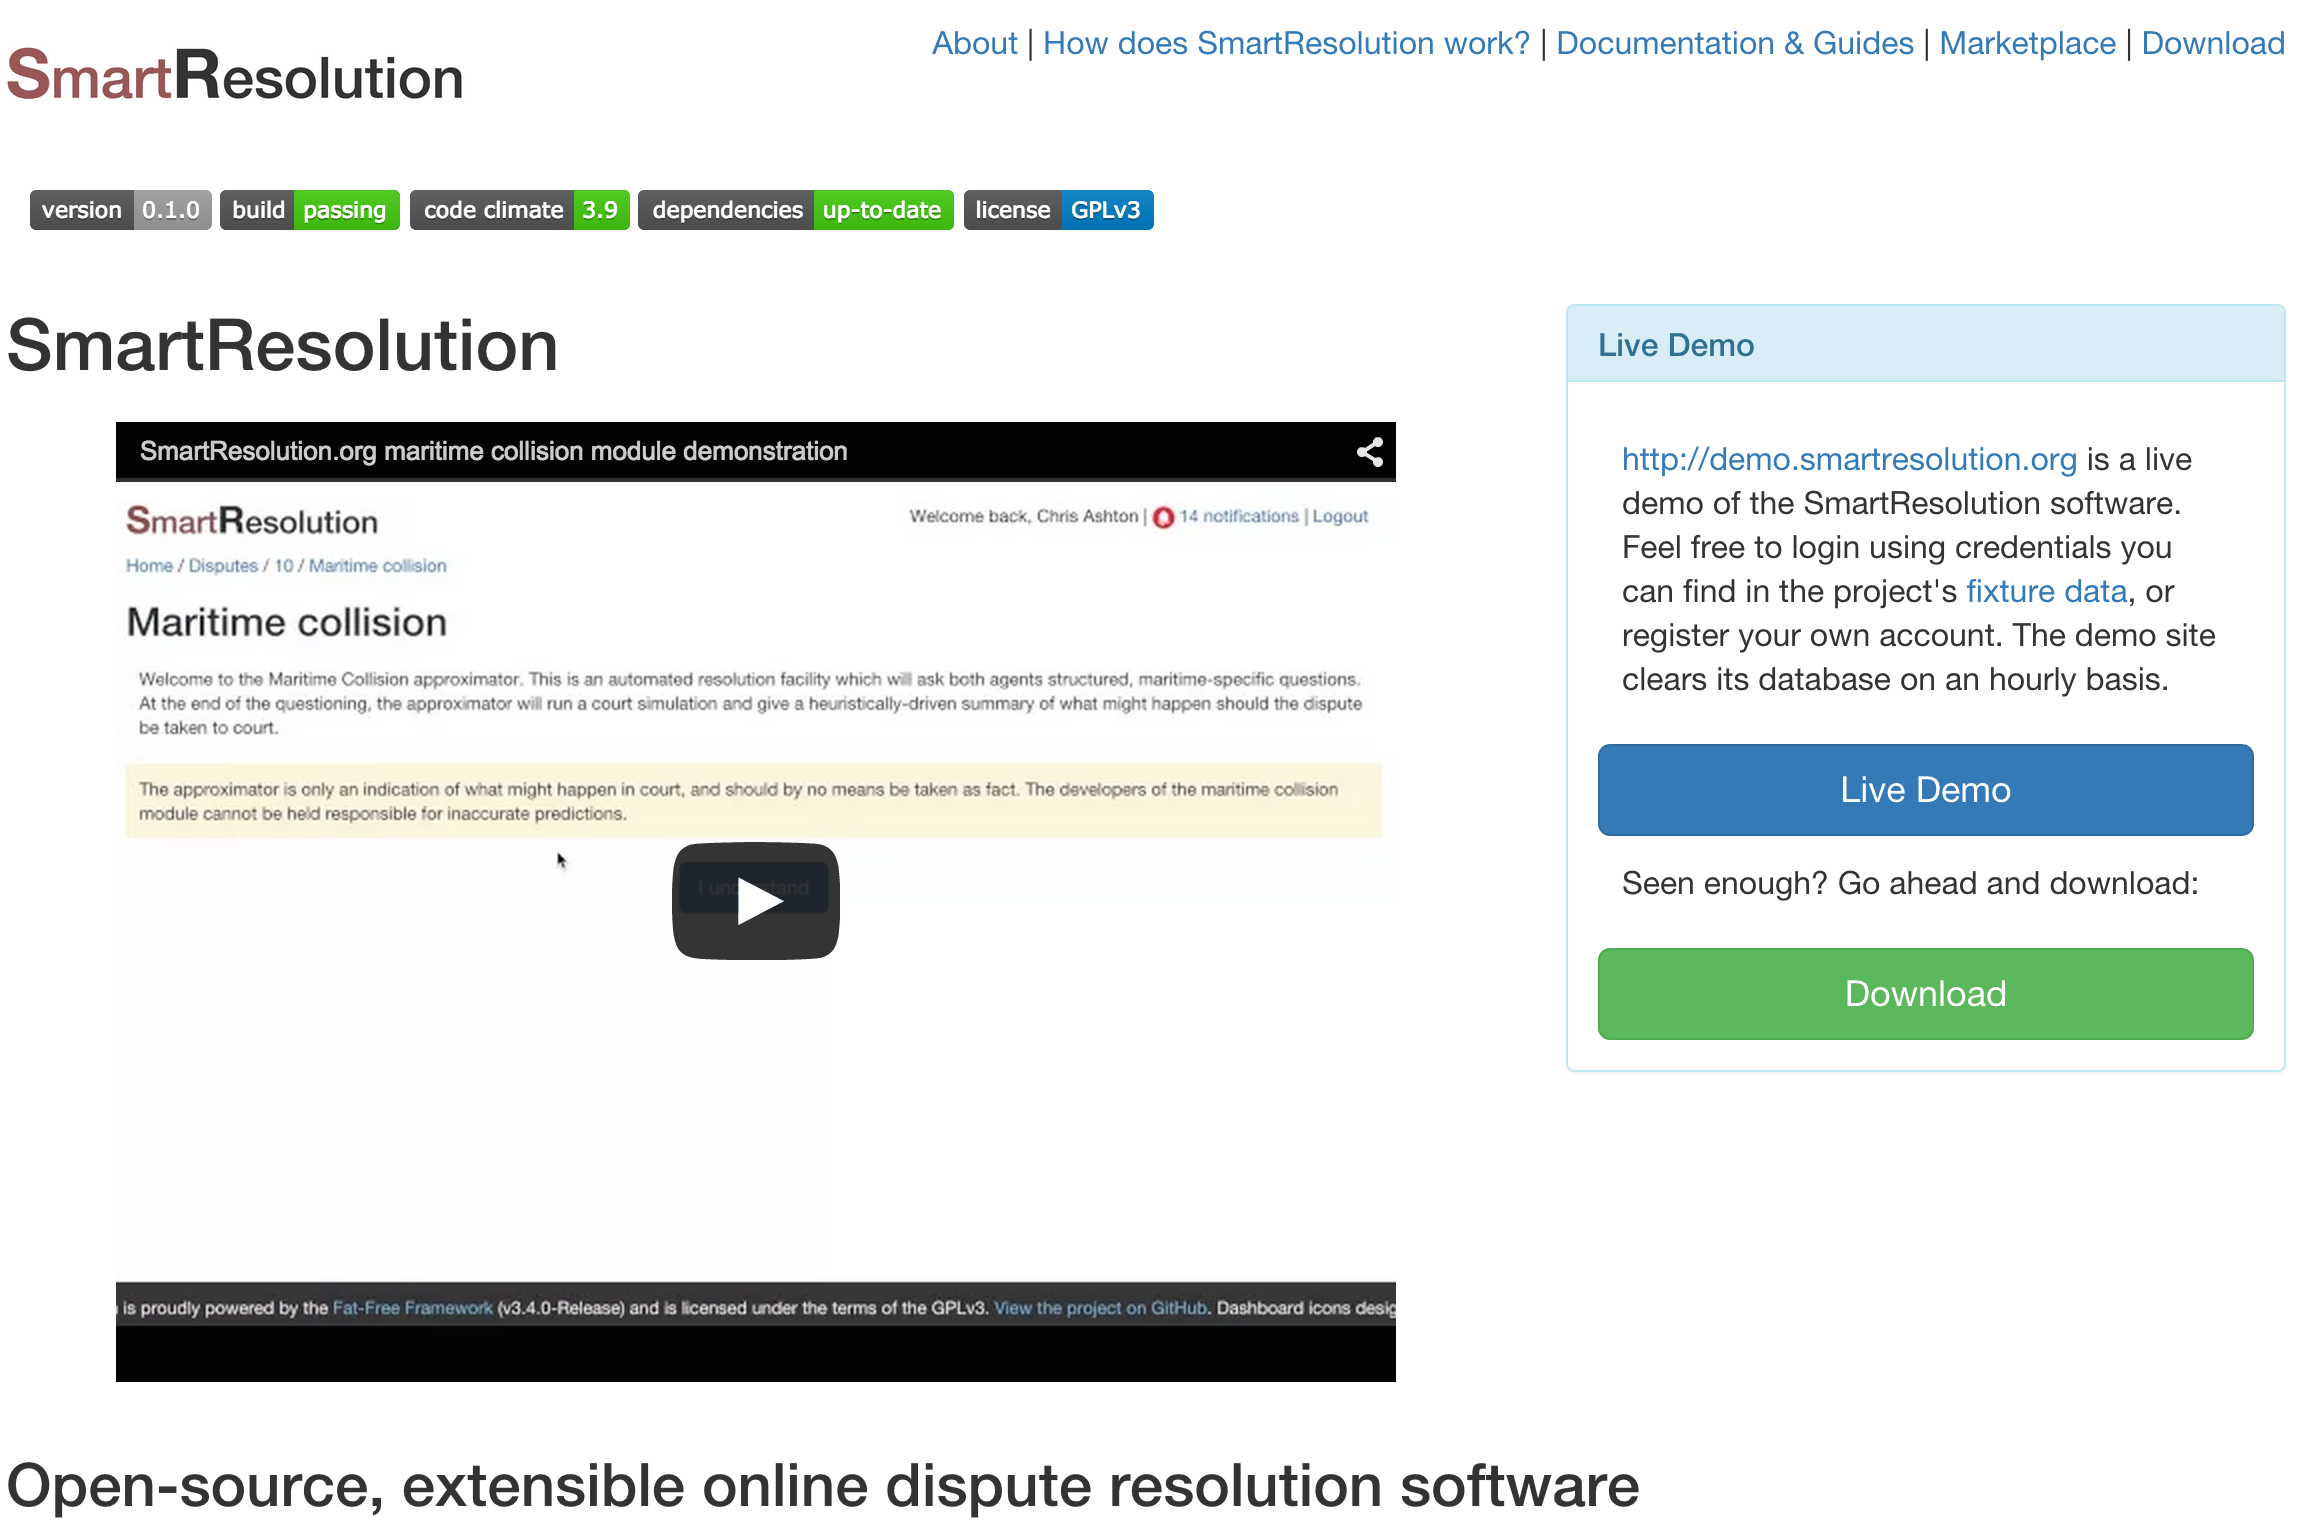
\includegraphics[width=\textwidth]{smartresolution--desktop}
    \fi
  \caption{Screenshot of SmartResolution vendor website in `desktop' view}
  \label{screenshot:smartresolutionOrg:desktop}
\end{figure}

Though responsiveness was not a requirement of the core SmartResolution software, I felt it was important to make the SmartResolution \emph{website} responsive. The website fulfils a different need and is likely to be stumbled upon by someone browsing on their phone, whereas lawyers using the SmartResolution \emph{software} are likely to be accessing it on a desktop or laptop at work.

Like the core platform, the website uses Bootstrap for the front-end, but it also uses the SlickNav JavaScript library to create the mobile navigation. Figure~\ref{screenshot:smartresolutionOrg:desktop} shows the landing page of the finished website. Figures~\ref{screenshot:smartresolutionOrg:tablet} and~\ref{screenshot:smartresolutionOrg:mobile} show the SmartResolution website responding to the viewport width, indicating how the website looks on a tablet and a mobile device respectively.

\begin{figure}[h!]
  \centering
    \ifimages
    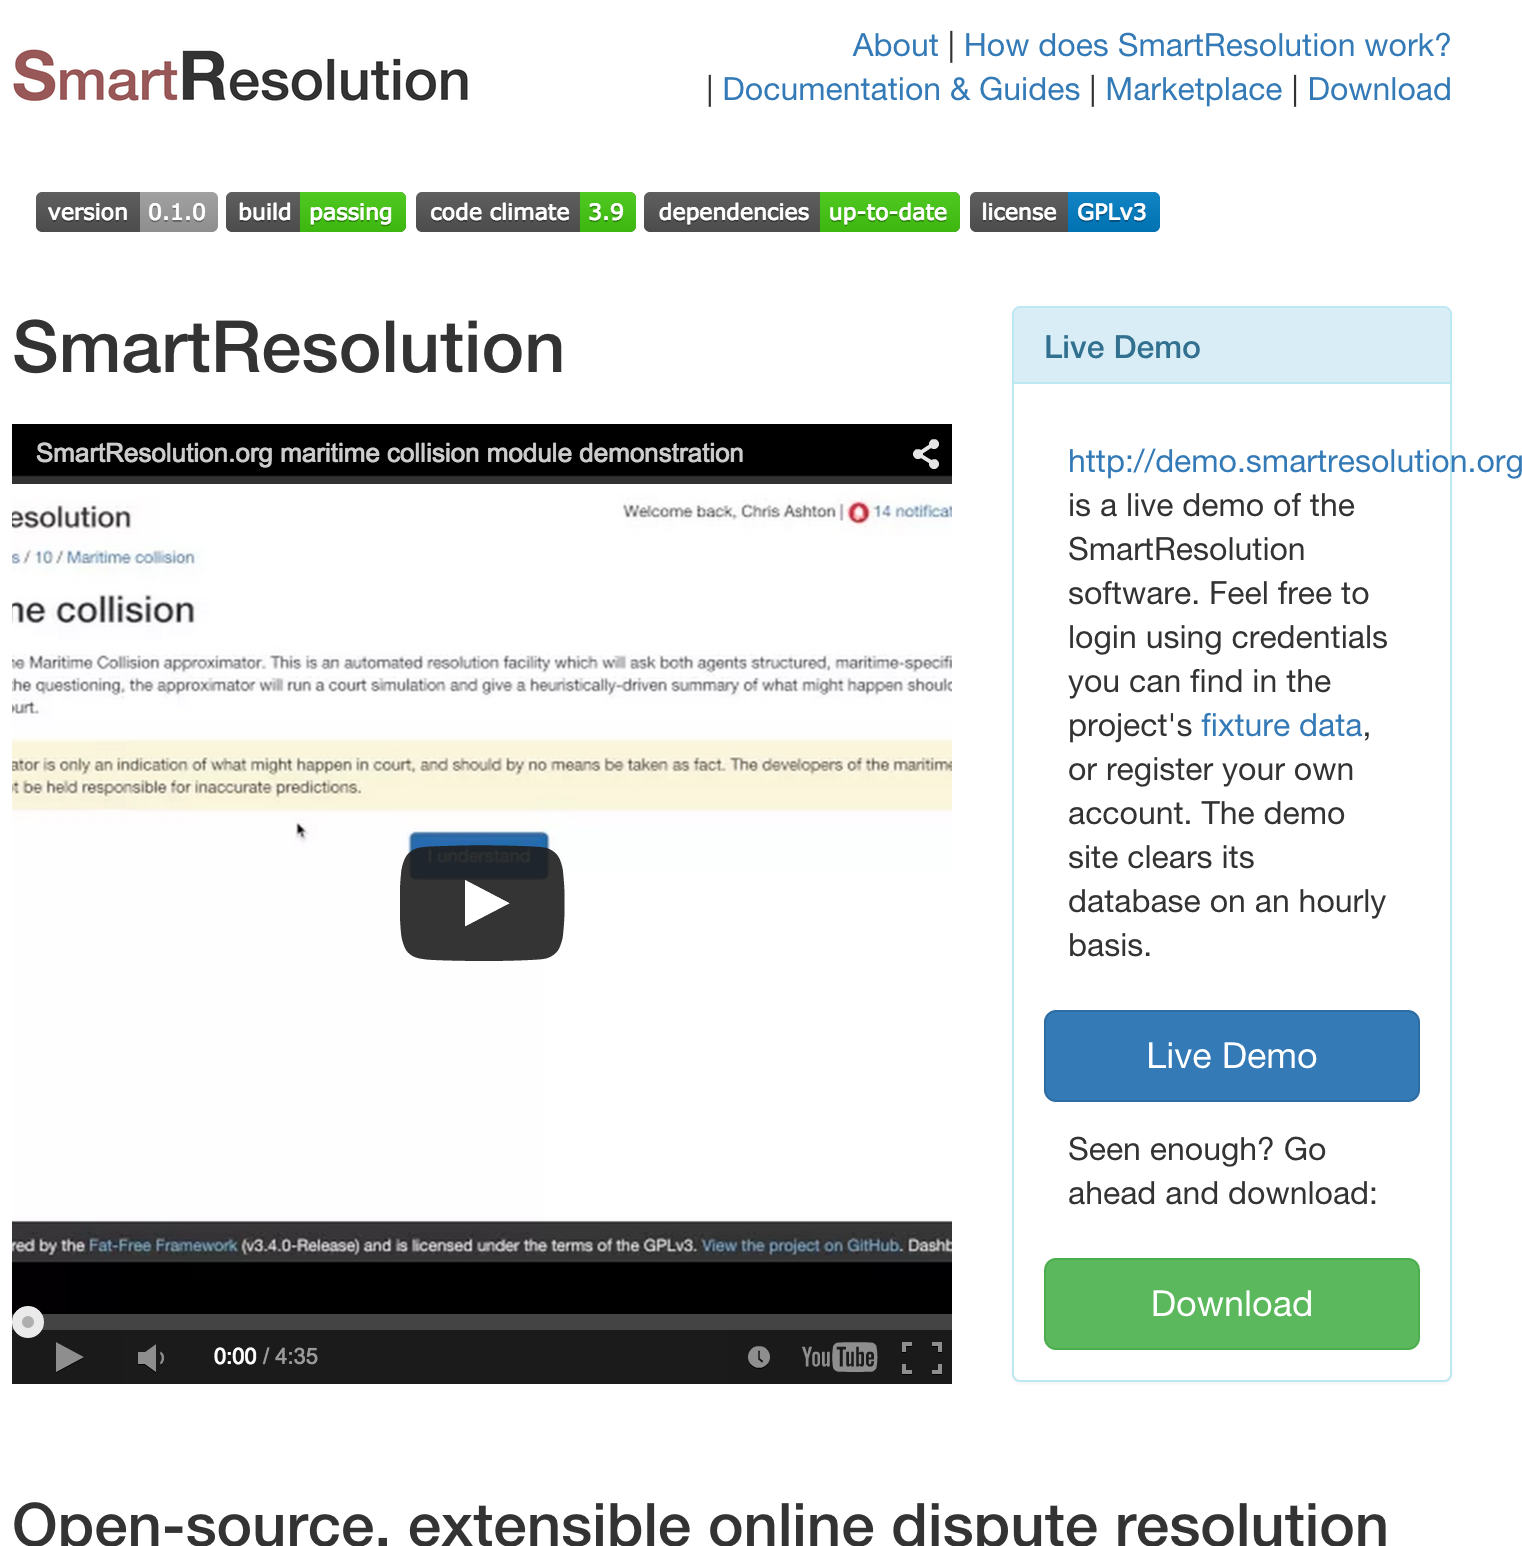
\includegraphics[width=\textwidth]{smartresolution--tablet}
    \fi
  \caption{Screenshot of SmartResolution vendor website in `tablet' view}
  \label{screenshot:smartresolutionOrg:tablet}
\end{figure}

\begin{figure}[h!]
  \centering
    \ifimages
    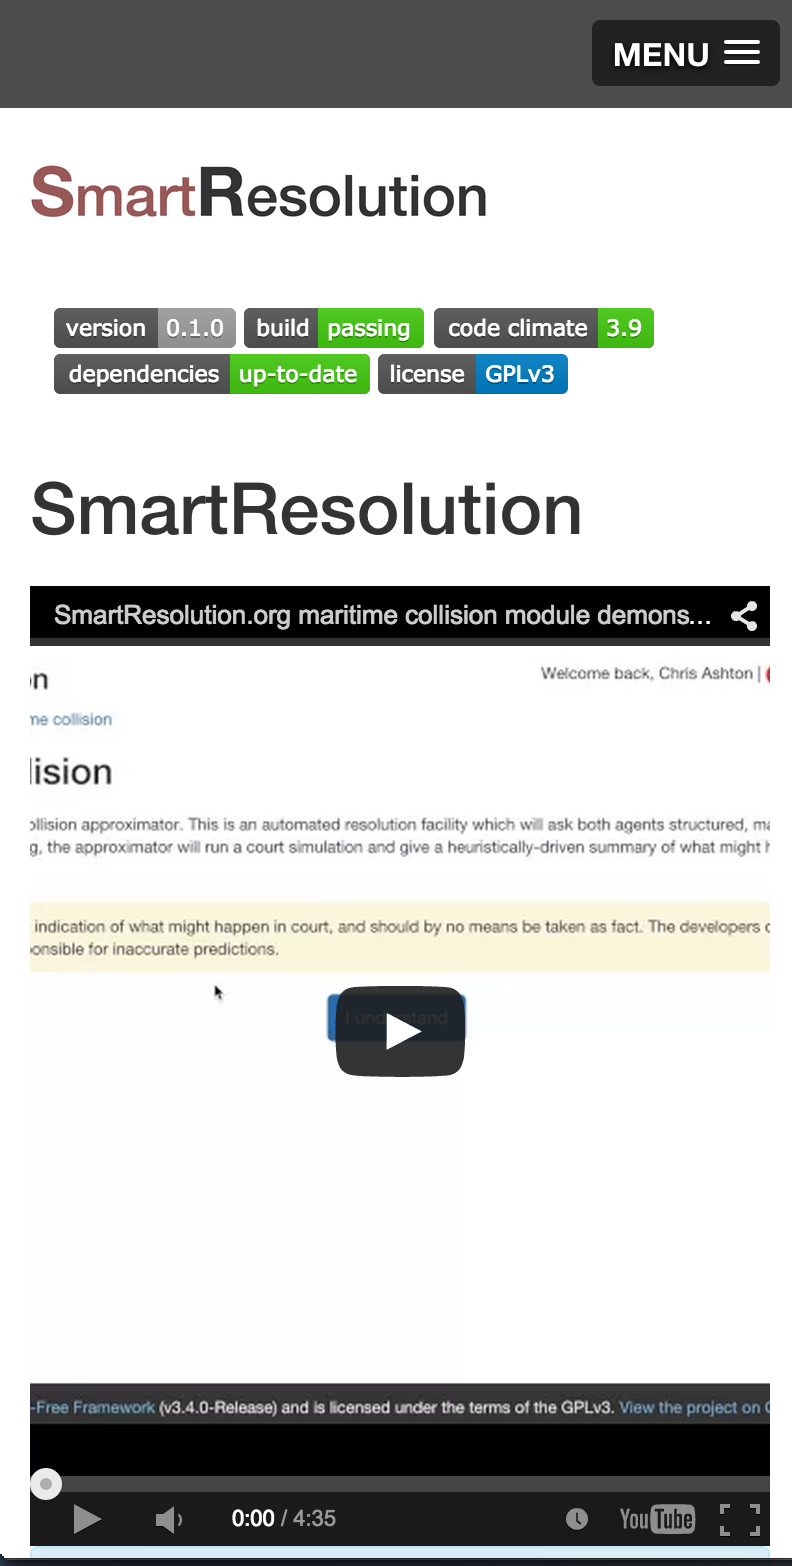
\includegraphics[width=0.5\textwidth]{smartresolution--mobile}
    \fi
  \caption{Screenshot of SmartResolution vendor website in `mobile' view}
  \label{screenshot:smartresolutionOrg:mobile}
\end{figure}

Though it would have been nice to have put the same effort into the core software, the size of the software would mean additional (and manual) testing time which could not be afforded on an aspect which was not a core requirement. Moreover, it was hoped that SmartResolution would eventually be able to support swappable themes: development effort would be better expended on that facility than on making sure the default theme is responsive.